\section{Systems Interactions}

%This section the interations flow of request for the system, by user create a new request into the system. The request flow is create by providing sequence diagrams, of demostration for 4 important task for the system, namely, register a user, user login, user create a new tweet, and user follow another user.
%
In figure \ref{fig:register_sequence}, \ref{fig:login_sequence}, \ref{fig:twit_sequence}, and \ref{fig:follow_sequence}, we show the flow of different user interactions.

\begin{figure}[H]
	\centering
	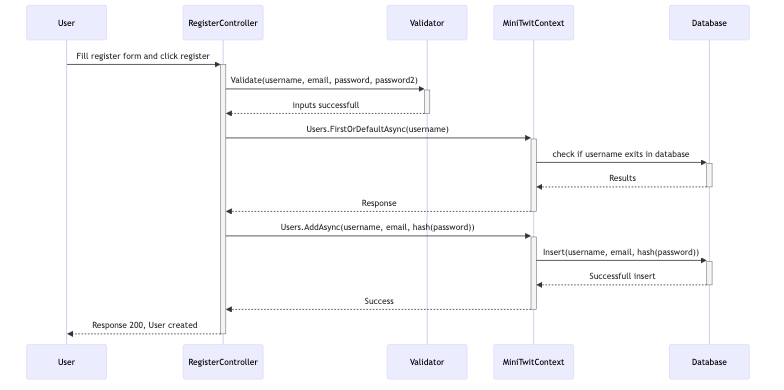
\includegraphics[width=0.75\textwidth]{register_sequence.png}
	\caption{Sequence diagram demostrate the flow of registerings of a user}
	\label{fig:register_sequence}
\end{figure}


\begin{figure}[H]
	\centering
	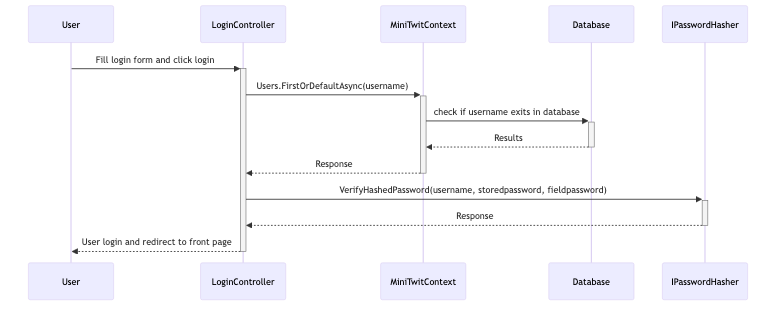
\includegraphics[width=0.75\textwidth]{login_sequence.png}
	\caption{Sequence diagram demostrate the login procedure for a user}
	\label{fig:login_sequence}
\end{figure}

\begin{figure}[H]
	\centering
	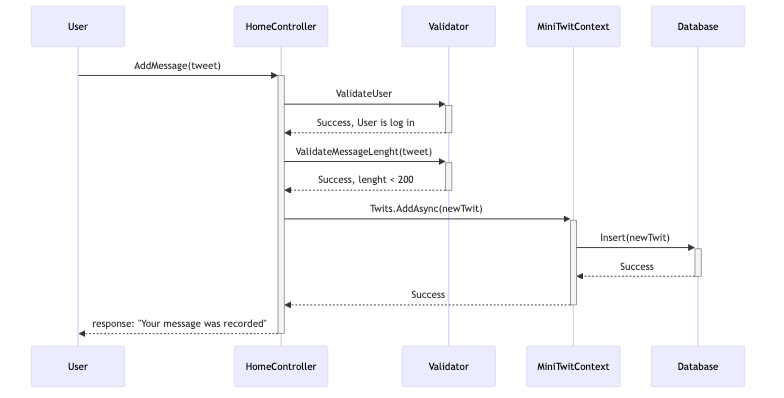
\includegraphics[width=0.75\textwidth]{twit_sequence.png}
	\caption{Sequence diagram demostrate the procedure for create a new twit}
	\label{fig:twit_sequence}
\end{figure}

\begin{figure}[H]
	\centering
	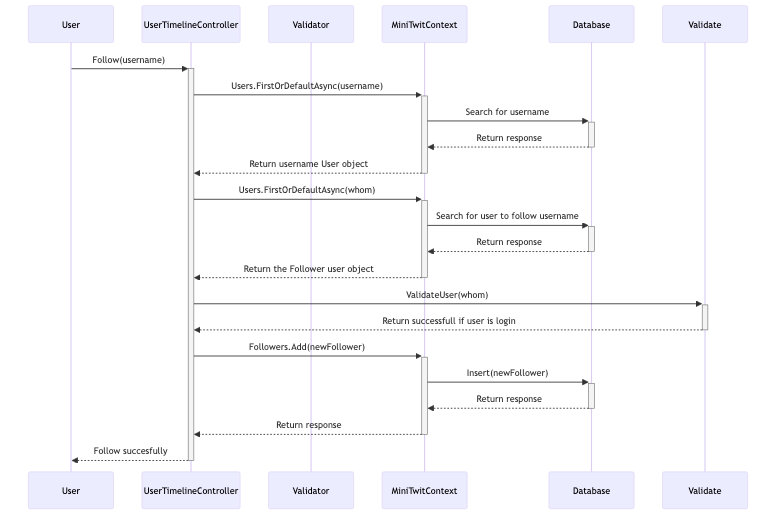
\includegraphics[width=0.75\textwidth]{follow_sequence.png}
	\caption{Sequence diagram of the procedure for a user follow another user}
	\label{fig:follow_sequence}
\end{figure}

